%	Use the standard preamble for Beamer slides of all 
%		statsTeachR modules
%		(\input, not \include, as \include can't access 
%		things in higher-level directories since it needs 
%		write permission there, which it doesn't have; and 
%		in some settings the preamble may be in a higher-level
%		directory than the source file.)
%	This path assumes the preamble is in the parent directory,
%		modify this if that changes.
%	************************************************
%	**	LaTeX preamble to be used with all 
%	**	statsTeachR labs/handouts.
%
%	Author: Eric A. Cohen
%	Last modified: 22 August 2013
%	************************************************

\documentclass[table]{beamer}

%	Set theme (a nice plain one)
\usetheme{Malmoe}

%	Use named colors, set main color of theme
%		to match Web site color:
\definecolor{MainColor}{RGB}{10, 74, 109}
\colorlet{MainColorMedium}{MainColor!50}
\colorlet{MainColorLight}{MainColor!20}
\usecolortheme[named=MainColor]{structure} 

%	For tables
%[dvipsnames] [table]
\usepackage{xcolor}
\usepackage{tabu}	% Even fancier than tabulary
\usepackage{multirow}

%	Just for the degree symbol
\usepackage{textcomp}

%	Get rid of footline (page, author, etc. on each slide)
\setbeamertemplate{footline}{}
%	Get rid of navigation buttons
\setbeamertemplate{navigation symbols}{}

%	Make footnotes not ugly
\usepackage{hanging}
\setbeamertemplate{footnote}{\raggedright\hangpara{1em}{1}\makebox[1em][l]{\insertfootnotemark}\footnotesize\insertfootnotetext\par}

%	Text style for code snippets inline in text:
\newcommand{\codeInline}[1]{\texttt{#1}}

%	Text style for emphasis stronger than \emph:
%		(Note, this doesn't toggle the way \emph does.
%			(Note, this can be done, didn't seem worth the trouble.))
\newcommand{\strong}[1]{{\bfseries{#1}}}


%	******	Define title page	**********************
\setbeamertemplate{title page}{
	{\color{MainColor}
	% There must be a better way than this -vspace at
	%	 the top and bottom of the page to reduce the 
	%	 bottom margin, but I can't find one that works.
	\vspace{-6em}

	% Go to a lot of trouble to get the title in a
	%	nice box, since customizing a beamer block
	%	does not entirely work here (I don't know why)
	\newlength{\titleBoxWidth}
	\setlength{\titleBoxWidth}{\textwidth}
	\addtolength{\titleBoxWidth}{-2.0em}
	\setlength{\fboxsep}{1.0em}
	\setlength{\fboxrule}{0pt}
	\fcolorbox{MainColor!25}{MainColor!25}{
		\parbox{\titleBoxWidth}{
			\raggedright
			\LARGE\textbf{\inserttitle}
		}	% end parbox
	}	% end fcolorbox

	\vfill
	\small{Author: \insertauthor}
	\vspace{\baselineskip}

	\small{\Course}

	\small{\Instructor}
	\vspace{\baselineskip}

	%\small{\emph{This material is part of the \strong{statsTeachR} project}}

	\vspace{0.33\baselineskip}\scriptsize{\emph{\LicenseText}}





		\vspace{-15em}

	}	% end color
	\clearpage
}	% end define title page



\usepackage{multicol}

%	The following variables are assumed by the standard preamble:
%	Global variable containing module name:
\title{Open Resources for Teaching Statistics }
%	Global variable containing module shortname:
%		(Currently unused, may be used in future.)
\newcommand{\ModuleShortname}{}
%	Global variable containing author name:
\author{Andrew Bray, Nicholas G Reich}
%	Global variable containing text of license terms:
\newcommand{\LicenseText}{Made available under the Creative Commons Attribution-ShareAlike 3.0 Unported License: http://creativecommons.org/licenses/by-sa/3.0/deed.en\textunderscore US }
%	Instructor: optional, can leave blank.
%		Recommended format: {Instructor: Jane Doe}
\newcommand{\Instructor}{UMass-Amherst Probability and Statistics Seminar Series}
%	Course: optional, can leave blank.
%		Recommended format: {Course: Biostatistics 101}
\newcommand{\Course}{7 April 2014}

\hypersetup{colorlinks=true, urlcolor=blue, linkcolor=black}



%	******	Document body begins here	**********************

\begin{document}

%	Title page
\begin{frame}[plain]
	\titlepage
\end{frame}

%	******	Everything through the above line must be placed at
%		the top of any TeX file using the statsTeachR standard
%		beamer preamble. 

%%%%%%%%%%%%%%%%%%%%%%%%%%%%%%%%

\begin{frame}{Many degrees of Openness}

\begin{multicols}{2}

\includegraphics[height = 1in]{OAlogo.png}

\columnbreak

\begin{block}{Common characteristics}
\begin{itemize}
        \item Online
\pause
	\item No access restrictions
\pause
	\item No cost
\pause
	\item Free-to-modify
\end{itemize}
\end{block}
\end{multicols}

\end{frame}



%%%%%%%%%%%%%%%%%%%%%%%%%%%%%%%%

\begin{frame}{Defining Open Access}

\begin{block}{Broadly...}
\begin{itemize}
        \item ``Free and unrestricted online availability'' (\href{http://www.budapestopenaccessinitiative.org/read}{Budapest Open Access Initiative})
        \item cf. ``Open source'' which typically describes only software
\end{itemize}
\end{block}

\begin{block}{In academia...}
\begin{itemize}
        \item Research: open-access publication options
        \item Teaching: open-access educational materials
\end{itemize}
\end{block}

\end{frame}

%%%%%%%%%%%%%%%%%%%%%%%%%%%%%%%%

\begin{frame}{The Open Access Education: a crowded field}

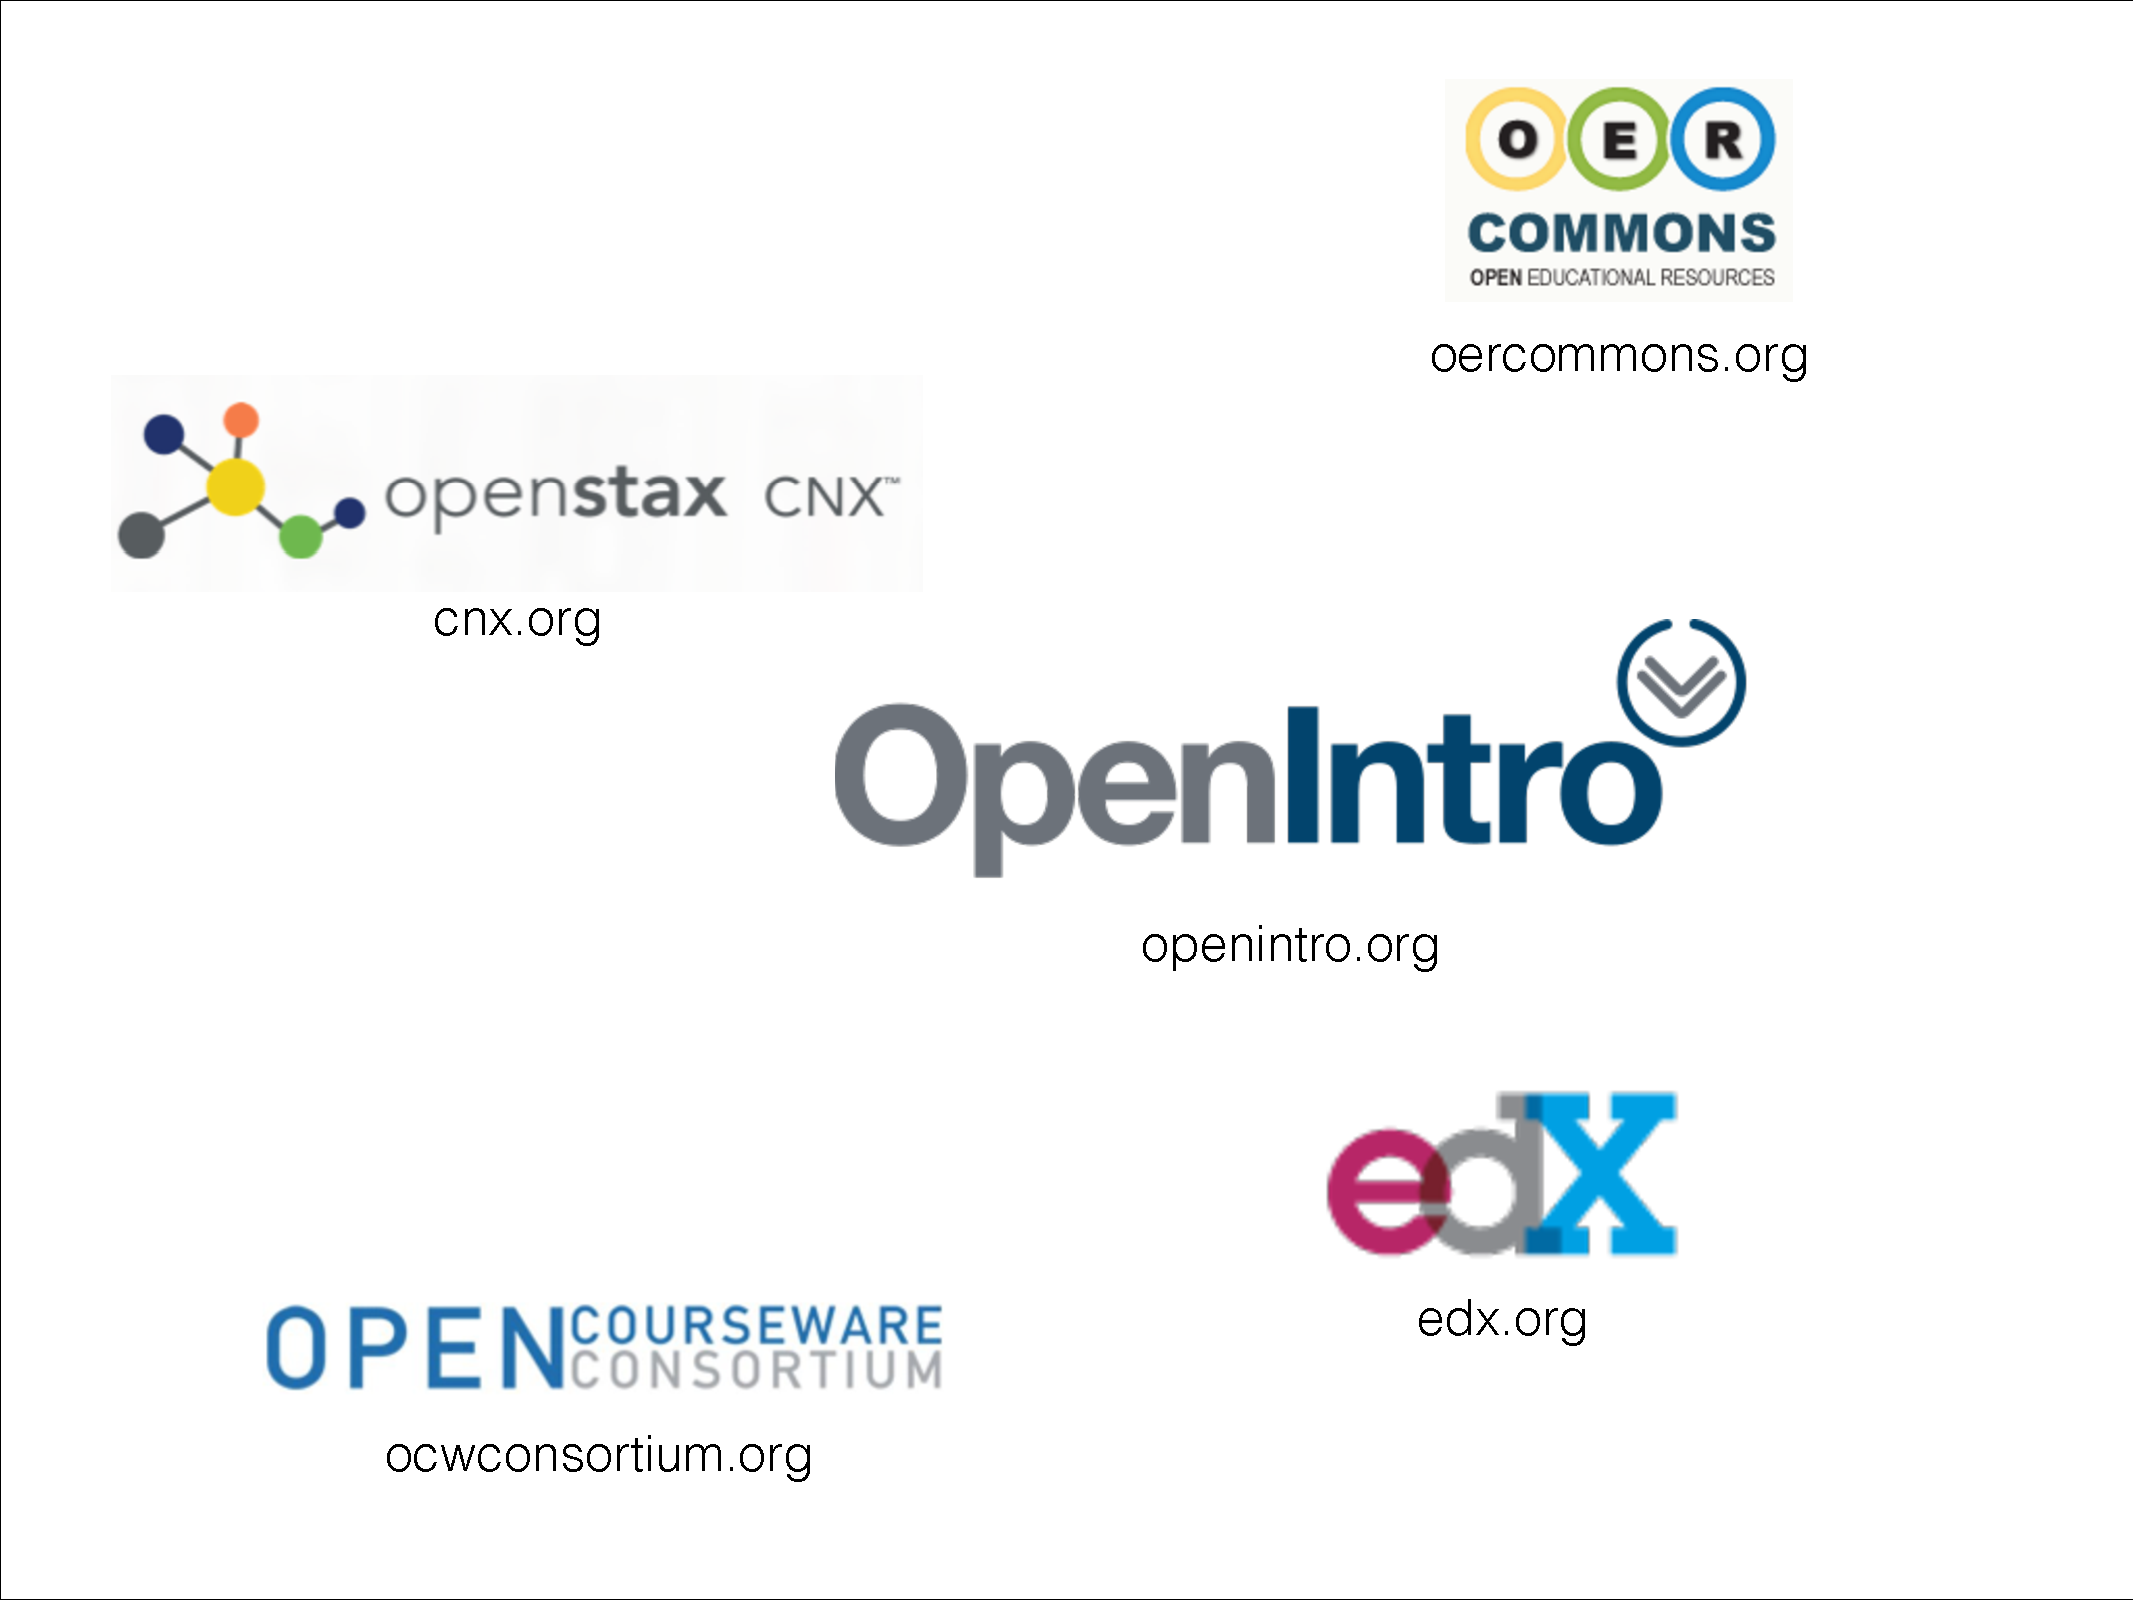
\includegraphics[width=\linewidth]{openEdLogos}

\end{frame}

%%%%%%%%%%%%%%%%%%%%%%%%%%%%%%%%

\begin{frame}{The Open Access Education: a governmental priority}

\begin{block}{Nov 2013: senate bill introduced}
\begin{itemize}
\item Senators Durbin, Franken Introduce Legislation to Help Make College Textbooks More Affordable

\item The \href{http://thomas.loc.gov/cgi-bin/query/z?c113:S.1704:}{Affordable College Textbook Act}: ``To expand the use of open textbooks in order to achieve savings for students.''
\end{itemize}
\end{block}

\begin{block}{January 2014: new NIH funding opportunity}
\begin{itemize}
\item \href{http://grants.nih.gov/grants/guide/rfa-files/RFA-HG-14-009.html}{NIH FOA} ``Open Educational Resources for Biomedical Big Data (R25)''
\item Designed to support ``Curriculum or Methods Development of innovative open educational resources that enhance the ability of the workforce to use and analyze biomedical Big Data.''
\end{itemize}
\end{block}

\end{frame}



%%%%%%%%%%%%%%%%%%%%%%%%%%%%%%%%

\begin{frame}{The Open Access Movement in Statistics}

\begin{block}{Many Statisticians see themselves as arbiters of science}
\begin{itemize}
\item many statisticians heralding reproducibility
\item reproducibile research often hinges on open access
\end{itemize}
\end{block}

\begin{block}{Many existing open-access stats textbooks}
\begin{itemize}
\item \href{http://www.openintro.org/stat}{OpenIntro}, by David Diez, Christopher Barr, Mina \c{C}etinkaya-Rundel
\item \href{http://www.math.umass.edu/~lavine/Book/book.html}{Introduction to Statistical Thought}, by Michael Lavine
\item \href{http://cnx.org/content/col10522/latest/}{Collaborative Statistics}, by Barbara Illowsky, Susan Dean
\item more listed on \href{http://www.openintro.org/stat/extras.php}{OpenIntro.org}
\end{itemize}
\end{block}

\end{frame}

%%%%%%%%%%%%%%%%%%%%%%%%%%%%%%%%

\begin{frame}{Many degrees of Openness}


\includegraphics[width=\linewidth]{FOASLogo.png}


{\footnotesize {\bf \em Philosophy} The mission of FOAS is to promote free software, open access publishing, and reproducible research in statistics. We understand free software to be as defined by the Free Software Foundation: possible to run for any purpose, available in source code form, and free to modify and/or redistribute. Open access forums for papers are, for us, defined as those that allow free access to all readers with an internet connection, and that invite contributions from authors without requiring the payment of fees. -- \href{http://www.foastat.org}{FOAStat.org}

%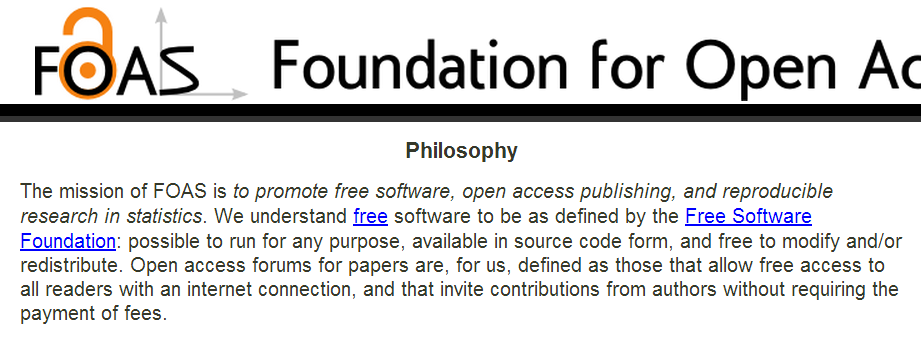
\includegraphics[height=1in]{FOAS.png}
}


\begin{itemize}
        \item Free software
\pause
	\item Open access publishing
\pause
	\item Open source educational resources
\end{itemize}

\end{frame}


%%%%%%%%%%%%%%%%%%%%%%%%%%%%%%%%


\begin{frame}{OpenIntro}

About 10 minutes of content

\end{frame}

%%%%%%%%%%%%%%%%%%%%%%%%%%%%%%%%


\begin{frame}{What is statsTeachR.org?}

\begin{block}{The basics}
\begin{itemize}
        \item a new, open-access, online repository with modular lesson plans
        \item materials targeted at undergraduates and graduates 
        \item topics: stats, biostats, statistical computing with R
\end{itemize}
\end{block}

\begin{block}{Modules}
\begin{itemize}
        \item each curricular ``module'' focuses on teaching a particular statistical subject or concept
        \item can be browsed \`a la carte
\end{itemize}
\end{block}

\end{frame}

%%%%%%%%%%%%%%%%%%%%%%%%%%%%%%%%

\begin{frame}{statsTeachR.org}

Website tour: \href{http://statsTeachR.org}{statsTeachR.org}

\end{frame}

%%%%%%%%%%%%%%%%%%%%%%%%%%%%%%%%

\begin{frame}{statsTeachR enables collaborative curriculum development}

\begin{block}{Some ongoing experiments for building curriculum}
\begin{itemize}
        \item graduate students are creating modules as final projects in core Biostat classes at UMass
        \item co-development of materials for similar classes (UMass-Amherst and Columbia Univ) 
\end{itemize}
\end{block}


\end{frame}

%%%%%%%%%%%%%%%%%%%%%%%%%%%%%%%%

\begin{frame}{Discussion questions}

\begin{itemize}
        \item where does the time/money/person-hours come from to generate these resources?
        \item how to incentivize these kinds of contributions appropriately?
        \item how to control quality of resources?
\end{itemize}
\end{frame}

%			\item draw distinction between open access publishing models and open source teaching materials
%                     \item resource challenges
%                     \item challenges of curation
%%%%%%%%%%%%%%%%%%%%%%%%%%%%%%%%


\end{document}